\chapter{METODOLOGI}
\label{sec:chap3_metodologi}

Penelitian ini dirancang dengan menggunakan serangkaian metode yang sistematis guna mencapai hasil re-identifikasi penyu laut yang akurat dan dapat digeneralisasi. Alur metodologi secara keseluruhan diilustrasikan melalui diagram berikut.

\begin{figure}[H]
    \centering
    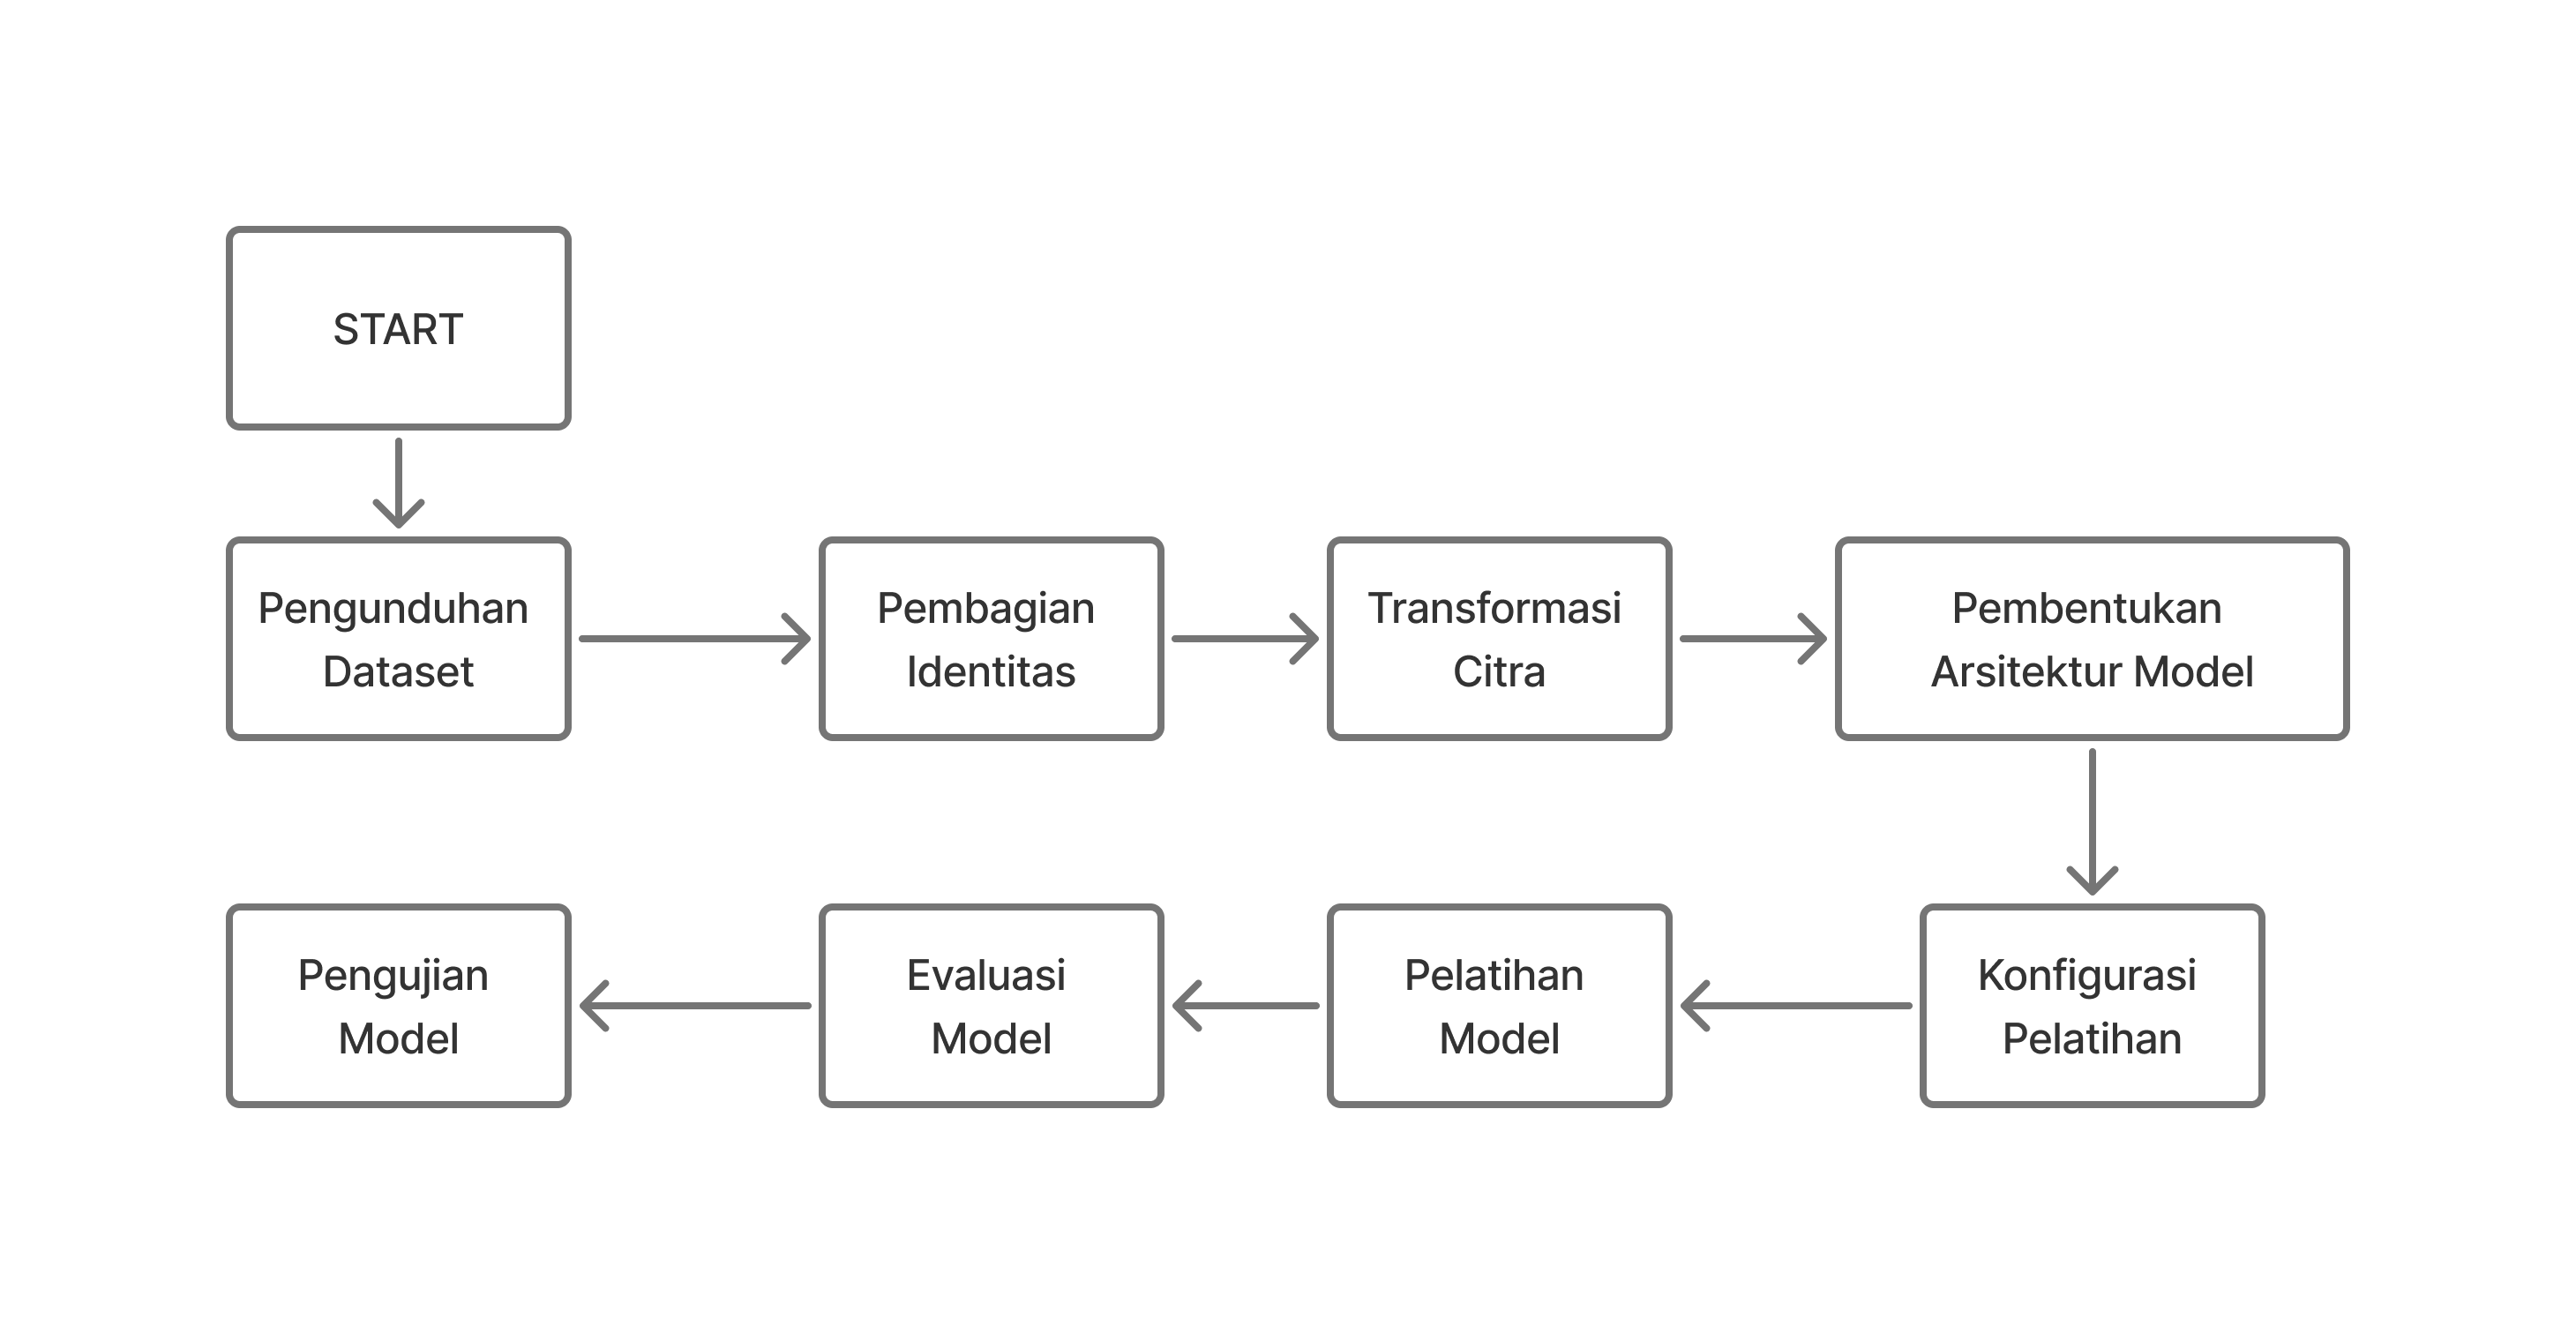
\includegraphics[width=0.9\linewidth]{bab3/diagram.png}
    \caption{Blok Diagram Pembangunan Model}
    \label{fig:diagram-block}
\end{figure}


\section{Dataset}
\subsection{Dataset SeaTurtleIDHeads}

Penelitian ini menggunakan dataset publik yang bernama \textit{SeaTurtleIDHeads}. Dataset \textit{SeaTurtleIDHeads} merupakan kumpulan data yang dirancang secara khusus untuk keperluan penelitian re-identifikasi individu penyu laut berdasarkan pola unik pada bagian kepala dan sisik mereka. Dataset ini banyak dimanfaatkan dalam bidang \textit{computer vision}, kecerdasan buatan, dan konservasi satwa liar, mengingat setiap individu penyu memiliki pola sisik kepala yang unik dan persisten sepanjang masa hidupnya, sebagaimana sidik jari pada manusia.

\begin{figure}[H]
    \centering
    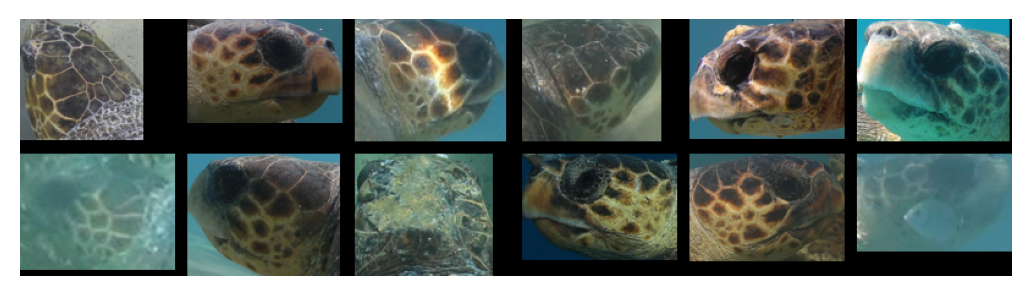
\includegraphics[width=0.9\linewidth]{bab3/SeaTurtleIDHeads.png}
    \caption{Sampel dataset SeaTurtleIDHeads \cite{wildlifedatasets_seaturtleidheads}}
    \label{fig:SeaTurtleIDHeads-sample}
\end{figure}

Dataset \textit{SeaTurtleIDHeads} memuat 7.582 citra dari 400 individu penyu laut yang dikumpulkan selama lebih dari satu dekade. Seluruh citra dalam dataset ini difokuskan pada bagian kepala penyu sehingga sesuai untuk digunakan dalam aplikasi identifikasi individu. Dataset ini memiliki variasi yang kaya dalam hal pose, pencahayaan, sudut pengambilan gambar, jarak kamera, dan resolusi citra, yang mencerminkan kondisi pengambilan foto secara nyata di lapangan. Variasi tersebut menjadi tantangan sekaligus peluang bagi model untuk mempelajari fitur yang benar-benar representatif terhadap identitas setiap individu.

Penelitian ini memilih \textit{SeaTurtleIDHeads} sebagai sumber data pelatihan dan validasi karena dataset ini menunjukkan keunggulan pada tugas re-identifikasi dibandingkan dengan anggota keluarga dataset yang sama, yaitu \textit{SeaTurtleID2022}. Dataset \textit{SeaTurtleID2022} memiliki resolusi citra yang lebih rendah dan dirancang terutama untuk tugas segmentasi, sehingga kurang ideal sebagai basis pelatihan bagi sistem re-identifikasi berbasis \textit{metric learning}.

\section{Pra-pemrosesan dan Augmentasi Data}
\subsection{Pembagian Dataset}

Dataset \textit{SeaTurtleIDHeads} dibagi menjadi tiga partisi menggunakan metode \textit{open-set identity split} dengan rasio 70:20:10, yang terdiri atas data pelatihan, data validasi, dan data pengujian. Pembagian dilakukan berdasarkan identitas individu sehingga tidak terdapat individu penyu yang sama pada lebih dari satu partisi. Hal ini memastikan bahwa evaluasi dilakukan terhadap identitas yang sepenuhnya belum pernah dilihat oleh model selama proses pelatihan (\textit{open-set evaluation}).

Sebelum pembagian dilakukan, identitas yang memiliki jumlah citra di bawah nilai minimum $N_{\min} = N_{\text{gallery}} + 2$ disaring dan dikeluarkan dari dataset. Persyaratan minimum tersebut memastikan bahwa setiap identitas memiliki citra yang cukup untuk dialokasikan ke galeri dan setidaknya dua citra ke \textit{query set}. Nilai parameter $N_{\text{gallery}}$ (yaitu $N_G$) merupakan salah satu variabel yang diuji dalam penelitian ini dan diuraikan lebih lanjut pada bab pengujian.

Data validasi dan data pengujian masing-masing dibagi lebih lanjut menjadi \textit{gallery set} dan \textit{query set}. Sebanyak $N_G$ citra per identitas dialokasikan ke galeri secara acak menggunakan \textit{random per-identity shuffle}, sementara sisa citra dialokasikan sebagai \textit{query}. Data validasi digunakan semata-mata untuk keperluan \textit{early stopping} dan pemilihan \textit{checkpoint} terbaik, sedangkan data pengujian hanya digunakan satu kali pada tahap evaluasi akhir.

\subsection{Transformasi Citra}

Seluruh citra diubah ukurannya menjadi $\mathit{img\_size} \times \mathit{img\_size}$ piksel sebelum dimasukkan ke dalam model. Nilai acuan $\mathit{img\_size} = 256$ digunakan sebagai \textit{baseline} dan merupakan salah satu variabel yang diuji dalam penelitian ini.

Pada fase pelatihan, diterapkan serangkaian augmentasi data yang berfungsi sebagai regularisasi implisit sekaligus meningkatkan kemampuan generalisasi model terhadap variasi kondisi pengambilan gambar. Augmentasi yang diterapkan meliputi hal-hal berikut.

\begin{itemize}
    \item \textbf{\textit{Random Crop}}: Citra diubah ukurannya menjadi $(\mathit{img\_size} + 32) \times (\mathit{img\_size} + 32)$ piksel, kemudian dipotong secara acak ke ukuran $\mathit{img\_size} \times \mathit{img\_size}$ piksel guna mensimulasikan variasi \textit{framing} dan posisi subjek.
    \item \textbf{\textit{Random Horizontal Flip}}: Citra dibalik secara horizontal dengan probabilitas 0,5, mengingat penyu dapat difoto dari sisi kiri maupun sisi kanan.
    \item \textbf{\textit{Color Jitter}}: Variasi acak diterapkan pada kecerahan, kontras, saturasi, dan \textit{hue} untuk mensimulasikan perbedaan kondisi pencahayaan bawah air.
    \item \textbf{\textit{Random Grayscale}}: Konversi citra ke format \textit{grayscale} dilakukan dengan probabilitas 0,1 untuk mendorong model agar tidak terlalu bergantung pada informasi warna.
    \item \textbf{\textit{Random Rotation}}: Rotasi acak diterapkan hingga 20 derajat guna mensimulasikan variasi sudut kamera.
    \item \textbf{\textit{Gaussian Blur}}: \textit{Blur} diterapkan menggunakan kernel berukuran $5 \times 5$ dengan nilai sigma acak antara 0,1 hingga 2,0 untuk mensimulasikan variasi fokus kamera.
    \item \textbf{\textit{Random Erasing}}: Area berbentuk persegi panjang dihapus secara acak pada citra dengan probabilitas 0,3 guna mensimulasikan oklusi parsial yang disebabkan oleh tumbuhan laut, bayangan, atau penghalang lainnya.
\end{itemize}

Pada fase evaluasi dan pengujian, hanya dilakukan operasi \textit{resize} dan normalisasi tanpa augmentasi acak agar hasil evaluasi bersifat deterministik dan dapat direproduksi.

Seluruh nilai piksel dinormalisasi menggunakan nilai rata-rata $\mu = (0{,}485,\ 0{,}456,\ 0{,}406)$ dan standar deviasi $\sigma = (0{,}229,\ 0{,}224,\ 0{,}225)$, yang merupakan statistik dari dataset ImageNet dan sesuai dengan statistik yang digunakan pada saat pra-pelatihan DINOv2.

\section{Arsitektur Model}

\subsection{Model Utama}

Arsitektur utama yang digunakan dalam penelitian ini adalah \textit{Vision Transformer} (ViT) yang telah dipra-latih menggunakan metode \textit{self-supervised learning} DINOv2. Model ini dimuat dari pustaka \textit{PyTorch Image Models} (timm). Model acuan yang digunakan adalah varian \textit{base}. Pada bab pengujian, akan dilakukan pelatihan menggunakan model lain dalam keluarga arsitektur yang sama.

ViT membagi citra masukan menjadi \textit{patch} berukuran $16 \times 16$ piksel. Untuk citra berukuran $256 \times 256$ piksel, terdapat $16 \times 16 = 256$ \textit{patch}. Setiap \textit{patch} diproyeksikan menjadi sebuah vektor dan diproses secara berurutan oleh 12 blok \textit{transformer}. Model ini menghasilkan keluaran berupa \textit{class token} berdimensi 768 yang merangkum representasi global dari keseluruhan citra.

DINOv2 dipilih sebagai metode pra-pelatihan karena terbukti menghasilkan representasi visual yang sangat kuat dan dapat ditransfer secara luas lintas domain tanpa memerlukan data berlabel. Pra-pelatihan berbasis \textit{self-distillation} ini mendorong model untuk mempelajari fitur semantik tingkat tinggi yang bersifat lokal maupun global, yang sangat relevan untuk tugas re-identifikasi di mana perbedaan antarindividu dapat bersifat sangat halus.

\subsection{Embedding Head}

Keluaran \textit{backbone} berupa vektor berdimensi 768 diproyeksikan ke dimensi \textit{embedding} yang lebih rendah menggunakan \textit{embedding head}. \textit{Head} ini terdiri atas tiga komponen yang diterapkan secara berurutan sebagai berikut.

\begin{enumerate}
    \item \textbf{\textit{Layer Normalization}}: Menormalisasi distribusi aktivasi dari \textit{backbone} sebelum proyeksi dilakukan. Langkah ini menstabilkan skala fitur yang masuk ke lapisan linear.
    \item \textbf{\textit{Dropout}}: Diterapkan dengan probabilitas $p_{\text{drop}}$ sebagai mekanisme regularisasi. Nilai acuan yang digunakan adalah $p_{\text{drop}} = 0{,}1$ dan merupakan salah satu variabel yang diuji dalam penelitian ini.
    \item \textbf{Proyeksi Linear}: Transformasi linear tanpa bias dari dimensi 768 ke dimensi \textit{embedding} $d_e$. Nilai acuan yang digunakan adalah $d_e = 256$ dan merupakan salah satu variabel yang diuji. Nilai ini dipilih karena proyeksi dengan dimensi 768$\rightarrow$768 tidak memberikan kompresi yang bermakna sehingga \textit{head} tidak dapat mempelajari representasi baru yang lebih diskriminatif.
\end{enumerate}

Setelah melewati \textit{head}, vektor dinormalisasi secara L2 sehingga seluruh \textit{embedding} berada pada permukaan \textit{unit hypersphere}. Normalisasi L2 tersebut memungkinkan penggunaan \textit{cosine similarity} yang setara dengan operasi perkalian titik, sehingga menyederhanakan proses perbandingan vektor pada tahap pengujian.

\subsection{ArcFace Loss}

ArcFace Loss digunakan sebagai fungsi \textit{loss} utama untuk pembelajaran separasi antaridentitas. ArcFace bekerja dengan menambahkan margin sudut $m_a$ pada sudut antara \textit{embedding} sampel dan bobot prototipe kelasnya di ruang bola satuan, sebelum penskalaan dengan faktor $s_a$ dan komputasi \textit{cross-entropy loss}.

Formulasi ArcFace Loss adalah sebagai berikut:
\begin{equation}
    \mathcal{L}_{\text{ArcFace}} = -\frac{1}{N} \sum_{i=1}^{N} \log \frac{e^{s_a \cdot \cos(\theta_{y_i} + m_a)}}{e^{s_a \cdot \cos(\theta_{y_i} + m_a)} + \sum_{j \neq y_i} e^{s_a \cdot \cos \theta_j}}
\end{equation}
di mana $\theta_{y_i}$ merupakan sudut antara \textit{embedding} sampel ke-$i$ dan bobot kelas yang benar $y_i$. Margin $m_a$ mendorong model untuk meningkatkan jarak sudut antara \textit{embedding} intra-kelas dan inter-kelas sehingga menghasilkan batas keputusan yang lebih tegas.

Pemilihan ArcFace dalam penelitian ini didasarkan pada beberapa pertimbangan. Pertama, sifat geometrisnya yang beroperasi pada bola satuan selaras dengan normalisasi L2 yang diterapkan pada keluaran \textit{embedding head}, sehingga seluruh proses pelatihan dan inferensi berlangsung dalam ruang yang konsisten secara geometris. Kedua, ArcFace telah terbukti efektif pada tugas re-identifikasi penyu secara spesifik, sebagaimana digunakan pada sistem \textit{baseline} \textit{SeaTurtleID2022} \cite{adam2023seaturtleid2022} maupun pada \textit{foundation model} MegaDescriptor \cite{cermak2024wildlifedatasets}, sehingga hasil yang diperoleh dapat dibandingkan secara langsung dengan penelitian terdahulu. Ketiga, kemampuan ArcFace dalam mempelajari representasi yang sangat diskriminatif dari kelas-kelas pelatihan sangat krusial mengingat perbedaan pola sisik antarindividu penyu dapat bersifat sangat halus.

Parameter yang diuji pada komponen ini adalah skala ArcFace $s_a$ dengan nilai acuan 64,0 dan margin ArcFace $m_a$ dengan nilai acuan 0,5.

\subsection{Online Hard Triplet Loss}

\textit{Triplet Loss} digunakan untuk memperkuat struktur lokal ruang \textit{embedding} melalui pembelajaran hubungan jarak relatif antarsampe. Setiap \textit{triplet} terdiri atas sebuah \textit{anchor} $a$, sebuah \textit{positive} $p$ (individu yang sama dengan \textit{anchor}), dan sebuah \textit{negative} $n$ (individu yang berbeda). Fungsi \textit{loss} ini mendorong terpenuhinya kondisi $d(a,p) + \text{margin} < d(a,n)$:

\begin{equation}
    \mathcal{L}_{\text{Triplet}} = \frac{1}{N} \sum_{i=1}^{N} \max\!\left(d(a_i, p_i) - d(a_i, n_i) + m_t,\ 0\right)
\end{equation}
di mana $d(\cdot, \cdot)$ adalah jarak Euclidean dan $m_t$ adalah margin \textit{triplet}.

Penelitian ini menggunakan strategi \textit{online hard mining}, di mana untuk setiap sampel dalam \textit{batch} dipilih \textit{positive} yang paling jauh (\textit{hardest positive}) dan \textit{negative} yang paling dekat (\textit{hardest negative}). Implementasi menggunakan \texttt{masked\_fill} untuk mengisolasi pasangan yang relevan, sehingga menghindari galat di mana nilai nol dari sampel yang bukan pasangan positif secara keliru terpilih sebagai jarak positif terkecil.

Parameter yang diuji pada komponen ini adalah margin \textit{triplet} $m_t$ dengan nilai acuan 0,3 dan bobot \textit{triplet} $\lambda_t$ dalam kombinasi \textit{loss} total dengan nilai acuan 0,5.

\subsection{Fungsi Loss Total}

Kedua fungsi \textit{loss} dikombinasikan secara linear sebagai berikut:

\begin{equation}
    \mathcal{L}_{\text{total}} = \mathcal{L}_{\text{ArcFace}} + \lambda_t \cdot \mathcal{L}_{\text{Triplet}}
\end{equation}
di mana $\lambda_t$ adalah bobot \textit{triplet}. Kombinasi ini memanfaatkan kelebihan masing-masing fungsi: ArcFace memberikan separasi global antarseluruh kelas yang terdefinisi di ruang proyeksi, sementara \textit{Triplet Loss} memperkuat konsistensi jarak lokal antara pasangan individu yang sama maupun berbeda pada setiap \textit{batch}.

\section{Konfigurasi Pelatihan}
\subsection{Balanced Batch Sampler}

Guna memastikan setiap \textit{batch} selalu memuat pasangan positif yang valid bagi \textit{Triplet Loss}, digunakan \textit{Balanced Batch Sampler}. Setiap \textit{batch} dibentuk dengan mengambil $P$ identitas secara acak, kemudian mengambil $K$ citra per identitas secara acak dengan penggantian (\textit{sampling with replacement}), sehingga ukuran \textit{batch} total adalah $P \times K$.

Nilai acuan yang digunakan adalah $P = 16$ identitas dan $K = 4$ citra per identitas, sehingga menghasilkan ukuran \textit{batch} sebesar 64. Nilai $P$ dan $K$ merupakan variabel yang diuji dalam penelitian ini. Identitas yang memiliki jumlah citra kurang dari $K$ dikeluarkan dari \textit{sampler} untuk menjaga konsistensi ukuran \textit{batch}.

Strategi ini lebih efektif dibandingkan dengan \textit{random sampling} konvensional, terutama pada dataset yang tidak seimbang. Dengan \textit{random sampling}, terdapat kemungkinan suatu \textit{batch} tidak memuat pasangan positif yang cukup, sehingga \textit{Triplet Loss} menjadi tidak informatif.

\subsection{AdamW dengan Layer-wise Learning Rate Decay}

Optimisasi dilakukan menggunakan AdamW dengan \textit{weight decay} $\lambda_w$ (nilai acuan: $10^{-4}$). AdamW dipilih karena memisahkan \textit{weight decay} dari pembaruan adaptif gradien, sehingga memberikan regularisasi yang lebih konsisten dibandingkan dengan Adam standar.

AdamW dikombinasikan dengan \textit{Layer-wise Learning Rate Decay} (LLRD) untuk melindungi representasi yang telah dipelajari selama pra-pelatihan DINOv2. LLRD memberikan \textit{learning rate} yang berbeda untuk setiap lapisan: lapisan yang lebih dalam (dekat dengan masukan) mendapatkan \textit{learning rate} yang lebih kecil, sedangkan lapisan yang lebih dekat ke keluaran mendapatkan \textit{learning rate} yang lebih besar.

Secara konkret, \textit{learning rate} untuk blok \textit{transformer} ke-$i$ (dari total $L = 12$ blok) dihitung menggunakan persamaan berikut:
\begin{equation}
    \eta_i = \eta_{\text{bb}} \cdot \gamma^{L - i}
\end{equation}
di mana $\eta_{\text{bb}}$ adalah \textit{backbone base learning rate} dan $\gamma$ adalah faktor peluruhan per lapisan. \textit{Embedding head} dan lapisan ArcFace menggunakan \textit{base learning rate} $\eta_{\text{base}}$ yang lebih tinggi, karena lapisan-lapisan tersebut diinisialisasi secara acak dan perlu belajar dengan laju yang lebih cepat.

Ketiga parameter tersebut, yaitu $\eta_{\text{base}}$, $\eta_{\text{bb}}$, dan $\gamma$, merupakan variabel yang diuji dalam penelitian ini dengan nilai acuan masing-masing sebesar $10^{-3}$, $10^{-5}$, dan $0{,}75$.

\subsection{Learning Rate Scheduler}

\textit{Learning rate scheduler} mengimplementasikan \textit{LambdaLR} yang membagi proses pelatihan menjadi dua fase berdasarkan fungsi skala $\lambda(e)$ terhadap \textit{epoch} $e$:

\begin{equation}
    \lambda(e) = \begin{cases}
        \dfrac{e + 1}{W} & \text{jika } e < W \quad \text{(fase \textit{warmup})} \\[10pt]
        \dfrac{1}{2}\!\left(1 + \cos\!\left(\pi \cdot \dfrac{e - W}{E - W}\right)\right) & \text{jika } e \geq W \quad \text{(fase \textit{cosine decay})}
    \end{cases}
\end{equation}
di mana $W$ adalah jumlah \textit{warmup epoch} dan $E$ adalah total jumlah \textit{epoch} pelatihan.

Pada fase \textit{warmup}, skala \textit{learning rate} meningkat secara linear dari $\frac{1}{W}$ menuju 1 selama $W$ \textit{epoch} pertama. Tujuannya adalah mencegah pembaruan gradien yang terlalu besar di awal pelatihan yang berpotensi merusak representasi DINOv2 sebelum \textit{embedding head} dan ArcFace mencapai kondisi yang stabil.

Pada fase \textit{cosine decay}, skala menurun dari 1 menuju 0 mengikuti kurva kosinus, sehingga memberikan penurunan \textit{learning rate} yang halus dan mencegah osilasi di sekitar titik minimum.

\subsection{Parameter Pelatihan Lainnya}

\begin{itemize}
    \item \textbf{\textit{Gradient Clipping}}: Norma gradien dibatasi pada nilai maksimum $G_{\max}$ (nilai acuan: 1,0) untuk menjaga stabilitas pelatihan dan mencegah terjadinya \textit{exploding gradient}.
    \item \textbf{Frekuensi Evaluasi}: Evaluasi pada data validasi dilaksanakan setiap 5 \textit{epoch}, bukan setiap \textit{epoch}, demi efisiensi komputasi.
    \item \textbf{\textit{Early Stopping}}: Proses pelatihan dihentikan lebih awal apabila tidak terdapat peningkatan nilai \textit{rank-1} pada data validasi selama $P_{\text{stop}}$ interval evaluasi berturut-turut (nilai acuan: 10 interval, setara dengan 50 \textit{epoch} tanpa peningkatan). \textit{Checkpoint} yang disimpan adalah model dengan nilai \textit{rank-1} validasi tertinggi.
    \item \textbf{\textit{Mixed Precision}}: Pelatihan menggunakan \textit{automatic mixed precision} (AMP) apabila GPU tersedia, guna mempercepat komputasi tanpa mengorbankan presisi numerik secara signifikan.
\end{itemize}

\section{Prosedur Pengujian}
\subsection{Ekstraksi Embedding}
\subsubsection{Aggregated TTA untuk Gallery}

Sebelum evaluasi dilakukan, seluruh citra dikonversi menjadi vektor representasi melalui proses \textit{embedding}. Proses ini dibedakan antara citra \textit{gallery} dan citra \textit{query}.

Citra \textit{gallery} diproses menggunakan \textit{aggregated TTA embedding}. Untuk setiap citra galeri, diterapkan 6 transformasi \textit{test-time augmentation} (TTA) yang berbeda, meliputi: (1) \textit{resize} standar, (2) \textit{center crop} dari ukuran yang lebih besar, (3) \textit{horizontal flip}, (4) \textit{center crop} yang lebih besar, (5) \textit{color jitter} kecerahan, dan (6) rotasi ringan diikuti \textit{crop}. Keenam \textit{embedding} yang dihasilkan kemudian dirata-ratakan dan dinormalisasi secara L2 sehingga menghasilkan satu vektor per citra galeri. Selanjutnya, vektor dari seluruh citra yang berasal dari identitas yang sama dirata-ratakan kembali dan dinormalisasi ulang, sehingga setiap entri galeri direpresentasikan oleh satu vektor tunggal yang lebih stabil dan andal dibandingkan dengan penggunaan \textit{embedding} dari satu citra tunggal.

\subsubsection{TTA untuk Query}

Citra \textit{query} diproses menggunakan protokol \textit{TTA embedding} yang sama: 6 augmentasi diterapkan pada setiap citra \textit{query}, kemudian \textit{embedding} dari keenam augmentasi dirata-ratakan dan dinormalisasi secara L2. Hasilnya adalah satu vektor \textit{embedding} per citra \textit{query}.

Konsistensi protokol TTA antara galeri dan \textit{query} merupakan hal yang krusial. Apabila hanya \textit{query} yang menggunakan TTA sementara galeri tidak, atau sebaliknya, distribusi vektor antara kedua set tidak akan sebanding sehingga dapat menurunkan akurasi pencarian.

\subsection{Evaluasi}
\subsubsection{Cosine Similarity}

Pada tahap pertama evaluasi, kemiripan antara setiap vektor \textit{query} dan seluruh vektor \textit{gallery} dihitung menggunakan \textit{cosine similarity}. Karena seluruh vektor telah dinormalisasi secara L2, operasi ini setara dengan perkalian matriks biasa:
\begin{equation}
    S = Q \cdot G^\top
\end{equation}
di mana $Q \in \mathbb{R}^{n_q \times d_e}$ adalah matriks \textit{embedding} \textit{query} dan $G \in \mathbb{R}^{n_g \times d_e}$ adalah matriks \textit{embedding} galeri. Setiap baris $S_i$ diurutkan secara menurun untuk mendapatkan peringkat kandidat identitas bagi \textit{query} ke-$i$.

\subsubsection{K-Reciprocal Re-Ranking}

Pada tahap kedua, diterapkan metode \textit{k-reciprocal re-ranking} untuk memperbaiki urutan hasil pencarian. Metode ini mengeksploitasi struktur hubungan timbal balik antartetangga terdekat di ruang \textit{embedding}: apabila dua sampel saling menjadi tetangga terdekat satu sama lain, keduanya memiliki kemungkinan besar berasal dari identitas yang sama.

Prosedur \textit{k-reciprocal re-ranking} adalah sebagai berikut:
\begin{enumerate}
    \item Seluruh vektor \textit{query} dan \textit{gallery} digabungkan, kemudian dicari $k_1$ tetangga terdekat untuk setiap sampel menggunakan FAISS (\textit{Facebook AI Similarity Search}) demi efisiensi komputasi.
    \item Himpunan \textit{k-reciprocal neighbors} $\mathcal{R}(i, k_1)$ dibangun. Sampel $j$ dimasukkan ke dalam $\mathcal{R}(i, k_1)$ apabila $i$ juga merupakan tetangga terdekat dari $j$. Himpunan ini selanjutnya diperluas dengan menambahkan tetangga dari tetangga (\textit{expansion}).
    \item Bobot afinitas $\mathbf{V}$ dihitung berdasarkan eksponensial negatif dari jarak, kemudian dihaluskan melalui \textit{query expansion} menggunakan $k_2$ tetangga terdekat.
    \item \textit{Jaccard distance} dihitung antara setiap pasang \textit{query}--\textit{gallery} berdasarkan irisan himpunan $\mathbf{V}$ yang bersesuaian.
    \item Jarak akhir dikombinasikan secara linear sebagai berikut:
    \begin{equation}
        D_{\text{final}}(q, g) = \lambda_{\text{rr}} \cdot D_{\text{cosine}}(q, g) + (1 - \lambda_{\text{rr}}) \cdot D_{\text{Jaccard}}(q, g)
    \end{equation}
    dengan nilai acuan $k_1 = 20$, $k_2 = 6$, dan $\lambda_{\text{rr}} = 0{,}3$.
\end{enumerate}

Hasil dari proses tersebut adalah matriks jarak yang telah diperbaiki, yang selanjutnya digunakan untuk menghitung ulang peringkat dan metrik evaluasi akhir.

\subsection{Metrik Evaluasi}

Dua metrik utama digunakan untuk mengukur performa sistem re-identifikasi:

\begin{itemize}
    \item \textbf{\textit{Cumulative Matching Characteristic} (CMC)}: Mengukur persentase \textit{query} yang identitas benarnya ditemukan dalam $k$ kandidat teratas. Metrik ini dilaporkan pada Rank-1, Rank-5, dan Rank-10. Rank-1 merupakan metrik yang paling penting karena mencerminkan akurasi identifikasi secara langsung tanpa intervensi manusia.
    \item \textbf{\textit{Mean Average Precision} (mAP)}: Mengukur rata-rata \textit{Average Precision} (AP) di seluruh \textit{query}. AP untuk satu \textit{query} memperhitungkan posisi seluruh citra galeri yang benar dalam daftar peringkat, bukan hanya yang pertama. mAP bersifat lebih informatif pada skenario di mana galeri memuat banyak citra per identitas.
\end{itemize}

Kedua metrik dihitung sebanyak dua kali: pertama berdasarkan urutan dari \textit{cosine similarity}, dan kedua berdasarkan urutan dari \textit{k-reciprocal re-ranking}.